\section{Experiment 2: Simulated Data with Latent Structure}

In the second simulation experiment, we focused on data generated from a Factor Analysis model.
The data social scientists analyse is often a collection of items measuring different latent constructs, 
a characteristic that is likely to impact imputation performances.
For Experiment 2, we considered three experimental factors.
First, the dimensionality of the data was controlled by the number of latent variables $l$ (10, 100).
5 items were generated as measurements of each latent variable, resulting in either 50 and 500 total items.
Second, factor loadings $\lambda_{ij}$ were defined as a 2-level random experimental factor (high, low).
High factor loadings were drawn from a uniform distribution between (0.9, 0.97), while low factor loadings
were drawn from a uniform distribution between (0.5, 0.6).
Third, the proportion of missing values was defined as a fixed experimental factor with two levels: 0.1 or 0.3.
Data with sample size $n=200$ were independently generated 1,000 times for each set of conditions.
Table \ref{tab:condExp2} summarizes the eight resulting conditions.
On each replicate, missing values were imposed and then each missing data treatment described in Section \ref{secMethods}
was used to obtain estimates for the parameters of a substantive analysis model of interest.
With a sample size fixed at 200, conditions with $l = 10$ resulted in a low-dimensional settings, while conditions 
with $l = 100$ resulted in a high-dimensional settings.

\begin{table}
	\centering
	\begin{tabular}{l | r | r | r | r | r }
		condition & n & p & l & pm & $\lambda$ range \\
		\hline
		1 & 200 & 50 &  10 &  0.1 & [.9, .97] \\
		2 & 200 & 500 & 100 & 0.1 & [.9, .97] \\
		3 & 200 & 50 &  10 &  0.3 & [.9, .97] \\
		4 & 200 & 500 & 100 & 0.3 & [.9, .97] \\
		5 & 200 & 50 &  10 &  0.1 & [.5, .6]  \\
		6 & 200 & 500 & 100 & 0.1 & [.5, .6]  \\
		7 & 200 & 50 &  10 &  0.3 & [.5, .6]  \\
		8 & 200 & 500 & 100 & 0.3 & [.5, .6]  \\
	\end{tabular}
	\caption{\label{tab:condExp2}Summary of conditions for experiment 2.}
\end{table}

\FloatBarrier % stops table:condSum leaving its own section

\subsection{Simulation Study Procedure}

%\paragraph{Data Generation}
	For each replication, an observed data matrix $\bm{Z}_{n \times p}$ was created based on a Confirmatory 
	Factor Analysis model.
	Each of $l$ latent variables was assumed to be measured by 5 items, for a total of $p = 5 \times l$ 
	columns in $\bm{Z}$.
	Values on the observed items for the $i$-th observation were obtained with the following measurement 
	model:
%
	\begin{equation}
		\bm{z}_i = \bm{\Lambda} \bm{\xi}_{i.} + \bm{\delta}_{i.}
	\end{equation}
%
	where $\bm{z}_i$ is a vector of $5*l$ observed items scores, for observations $i = 1, ..., n$;
	$\bm{\Lambda}$ is the $(5*l) \times l$ matrix of factor loadings; $\bm{\xi}_{i.}$ is a vector of $l$ latent scores 
	for observation $i$; and $\bm{\delta}_{i.}$ is a vector of $5*l$ uncorrelated measurement errors sampled from a 
	multivariate normal distribution centered around a mean vector of 0s and with a diagonal covariance matrix $\bm{\Theta}$.
	All items are centered around a mean of 5.
	For notation and model specification the interested reader may refer to \cite{bollen:1989}.

	The latent scores in $\bm{\xi}_{i.}$ are sampled from a multivariate normal distribution centered around 
	0, and with a covariance matrix $\bm{\Psi}$, with diagonal elements equal to 1 and off-diagonal elements 
	equal to correlation between latent factors. 
	In particular, the first 4 latent variables are highly correlated ($\rho = .6$), the second block of 4 
	latent variables are weakly correlated ($\rho = .3$), while the remaining $l-8$ latent variables are 
	uncorrelated.

	The matrix $\bm{\Lambda}$ defines a simple latent structure where each item loads on only 1 factor (5 items 
	for each latent variable).
	Both the item and latent factor variances are set to 1 so that the measurement error variance is defined as 
	$var(\delta) = 1 - \lambda^{2}$.
	This specification allows factor loadings $\lambda_{ij}$, with $i = 1, ..., n$ and $j = 1, ..., l$, to be
	defined as standardized values between 0 and 1.
	If all values in $\bm{\Lambda}$ are 0s, there is no latent structure and items are simply drawn from a
	multivariate normal distribution centered around the item means with covariance matrix $\bm{\Theta}$.
	If all values in $\bm{\Lambda}$ are 1s, there is a \emph{perfect} latent structure, meaning that items
	exactly measure the latent constructs.
	The exact values for the latent factors are drawn for each repetition from a uniform distribution between
	lower $b_l$ and upper bound $b_u$, that are condition-specific (see below).

%\paragraph{Missing Data Imposition}

	Item non-response was imposed on 10 items in $\bm{Z}_{n \times p}$.
	The items targeted by the missing data measured two highly correlated latent variables ($l = 1, 2$).
	The same strategy described in Subsection \ref{sub_missing} was used.	
	The predictors included in $\tilde{Z}$ (see Equation \ref{eqn:rm}) were the latent scores for the other two highly 
	correlated latent variables ($l = 3, 4$).
	
%\paragraph{Imputation}
	
	Missing values were treated according to all the methods described in Section \ref{secMethods}.
	The imputation methods were parametrized as in Experiments 1.
	50 iterations were sufficient for convergence for all MI methods except blasso, which required approximately 
	2000 iterations for convergence.

%\paragraph{Analysis}
	
	The substantive model of interest in Experiment 1 was a saturated model that estimates means,
	variances, and covariances of the items with missing values.
	Furthermore, the true Factor Analysis model for the same items was estimated to see how the 
	factor loadings were recovered after imputation.

\subsection{Results}
	The same comparison criteria defined in Subsection \ref{criteria} were used to assess the performances of 
	the methods.
	Figures \ref{fig:exp2bias14} and \ref{fig:exp2cir14} report the average, minimum, and maximum PRB and CIC obtained
	with each missing data treatment method for each parameter type (means, variances, and covariances) in the 
	conditions with high factor loadings.
	Figures \ref{fig:exp2bias58} and \ref{fig:exp2cir58} report the same results for the conditions with low 
	factor loadings.
	In the supplementary material you may find the figures reporting the PRBs and CICs for every parameter.

	\paragraph{Means}
	All the imputation methods provided unbiased estimates of the item means with PRBs that were almost 0 
	for all items.
	For high proportion of missing cases (column 3 and 4) there was a slight increase in PRB values for 
	all methods except IURR, bridge, and MI-PCA.
	However, only Complete Case analysis led to unacceptable bias of the means.
	DURR, IURR and MI-PCA resulted in little to no deviations from nominal coverage in all conditions, 
	while blasso, MI-CART, MI-RF, bridge, and missForest led to significant under-coverage of the true means when the 
	proportion of missing cases was high (columns 3 and 4).
	
	\paragraph{Variances}
	All MI methods, except Bridge, resulted in acceptable estimation bias for the item variances in all conditions, 
	but the least biased estimates were obtained by MI-OP, IURR and MI-PCA.
	CIC decreased as the proportion of missing cases increased (from condition 1 and 2 to conditions 3 and 4).
	For high $pm$, only IURR and MI-PCA maintained CICs mostly within the range .94-.96, while blasso and the MI tree-based 
	methods led to mild to extreme under-coverage (all CICs < 90\%).
	Single data approaches, missForest and CC, showed again extreme (negative) bias and CI under-coverage in 
	almost all conditions.

	The large positive bias (and low CIC) for the item variances that afflicted MI-PCA in the multivariate-normal set up 
	(Figures \ref{fig:exp1bias} and \ref{fig:exp1cir}) is not present in figures \ref{fig:exp2bias14} and \ref{fig:exp2cir14}.
	However, that pattern reappeared when the factor loadings were small, as can be seen in Figure \ref{fig:exp2bias58} 
	and \ref{fig:exp2cir58}.

	\paragraph{Covariances}
	For all the conditions with high factor loadings in experiment 2, IURR and DURR showed acceptable covariance biases 
	($|\text{PRB}|<10\%$).
	However, they led to large negative bias in all the conditions with low factor loadings (see Figures \ref{fig:exp2bias58} 
	and \ref{fig:exp2cir58}).
	The other methods followed the same pattern as in experiment 1: the MI-PCA approach resulted in the lowest 
	bias and deviation from nominal coverage for the covariances of the observed items; 
	all other methods led to large negative biases and mild-to-extreme under-coverage for all the covariances, 
	in all conditions.

\begin{figure}
	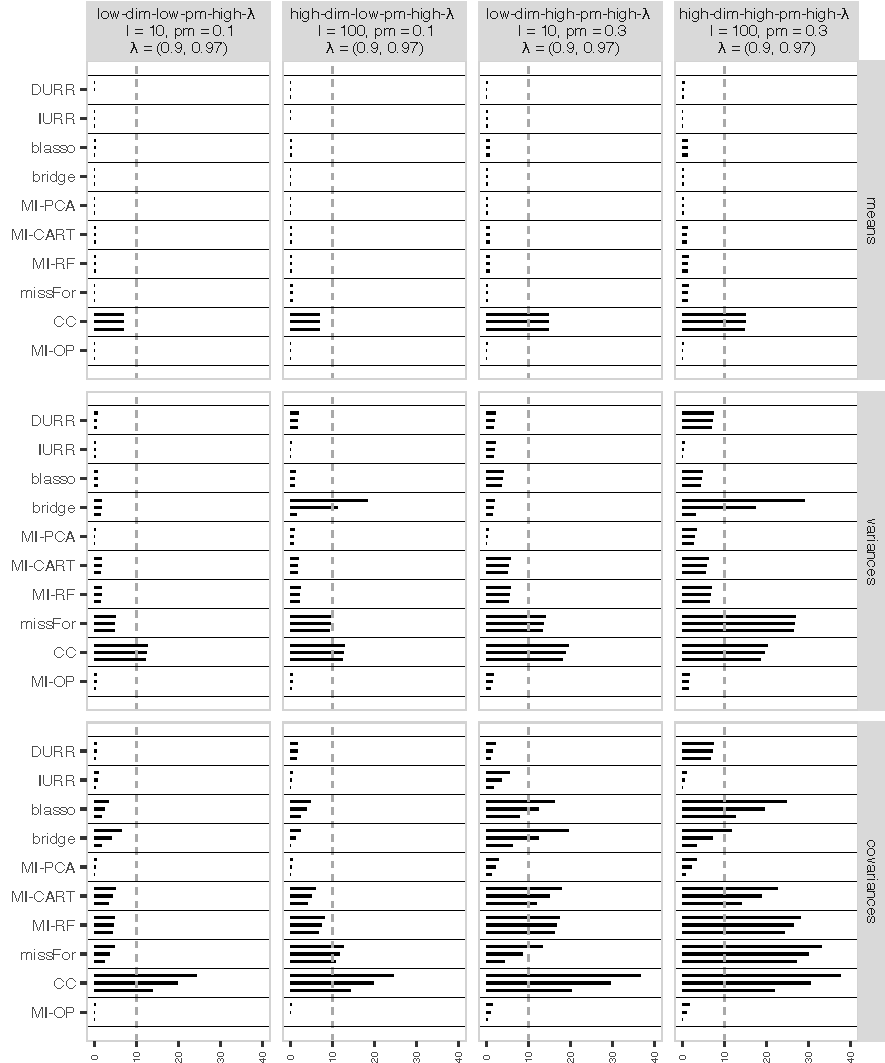
\includegraphics{../../output/graphs/exp2_semR_bias_14_summy.pdf}
\caption{PRBs for the means, variances and covariances (PRB) for condition 1 to 4.
	For every method, single horizontal lines, representing the PRB of a parameter estimate on 
	a single variable (or pair of variables), combine to form larger horizontal bars giving an 
	aggregate account of how each method performed across multiple variables with missing values.
}
\label{fig:exp2bias14}
\end{figure}

\begin{figure}
	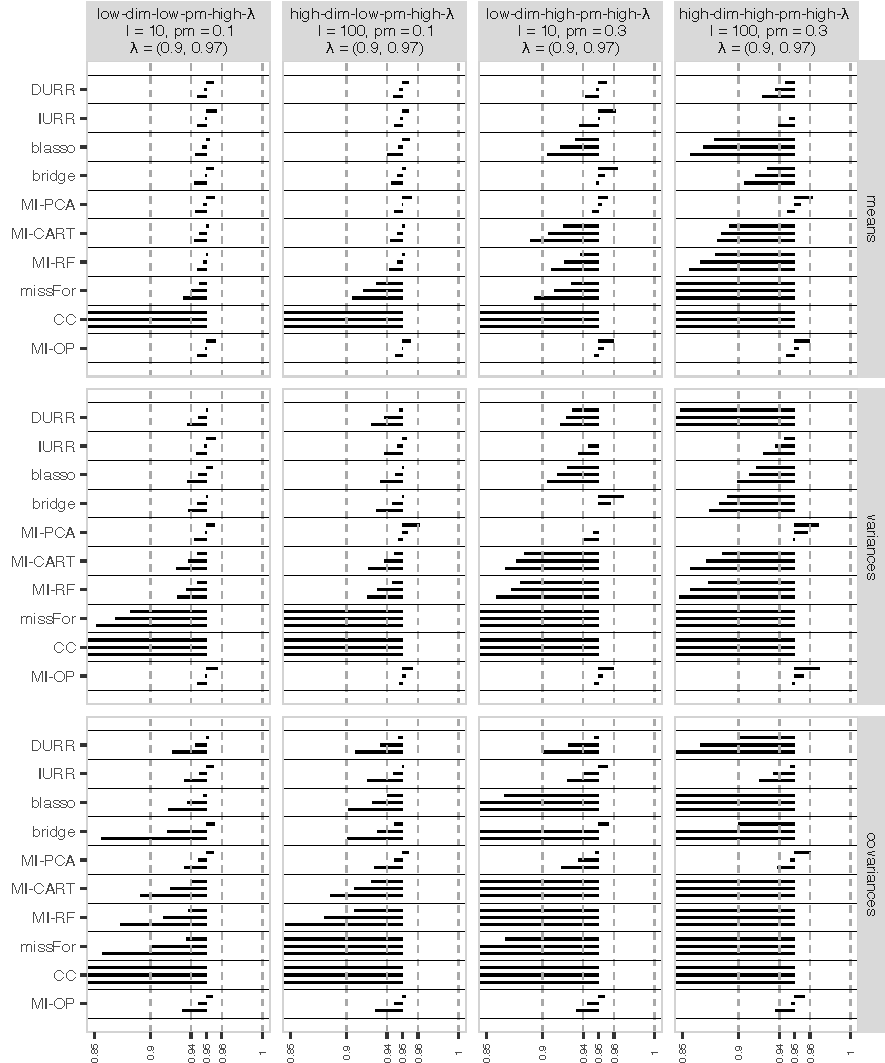
\includegraphics{../../output/graphs/exp2_semR_ci_14_summy.pdf}
\caption{CIC for the means, variances, and covariances for condition 1 to 4.
	For every method, single horizontal lines, representing the CIC of a parameter estimate on 
	a single variable (or pair of variables), combine to form larger horizontal bars giving an 
	aggregate account of how each method performed across multiple variables with missing values.
}
\label{fig:exp2cir14}
\end{figure}

\begin{figure}
	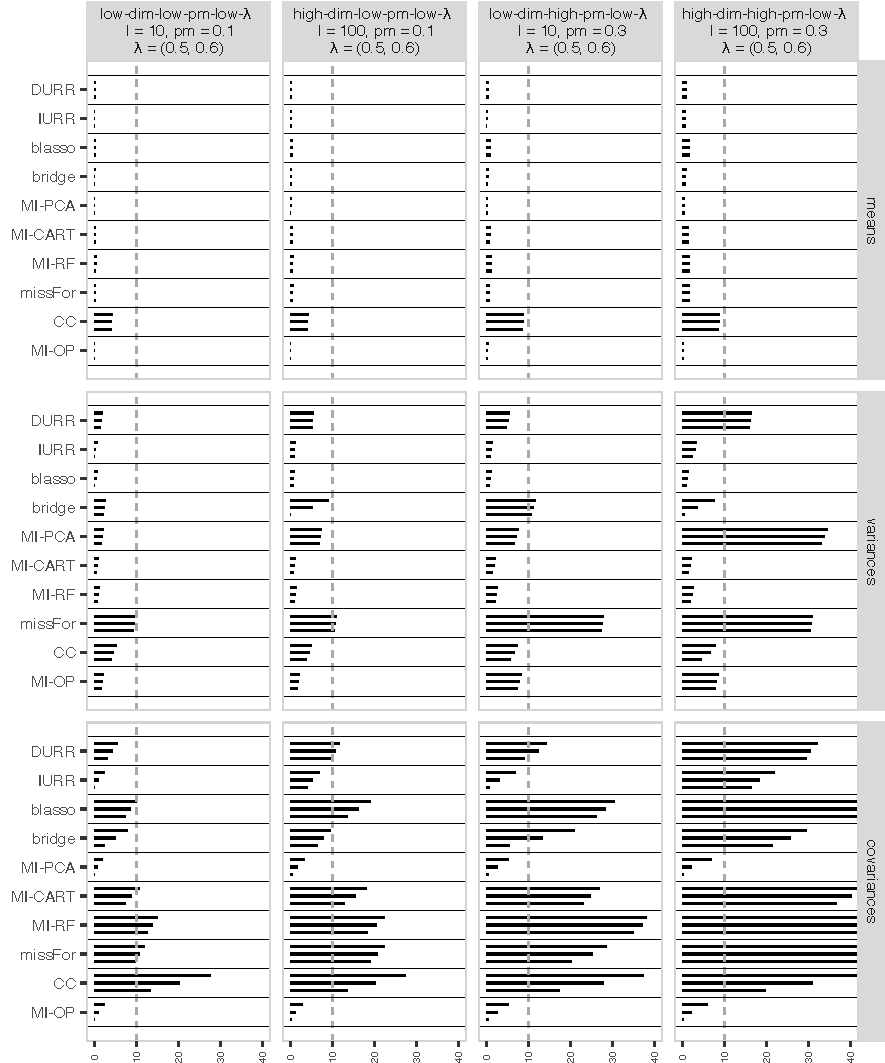
\includegraphics{../../output/graphs/exp2_semR_bias_58_summy.pdf}
\caption{PRBs for the means, variances and covariances (PRB) for condition 1 to 4.
	For every method, single horizontal lines, representing the PRB of a parameter estimate on 
	a single variable (or pair of variables), combine to form larger horizontal bars giving an 
	aggregate account of how each method performed across multiple variables with missing values.
}
\label{fig:exp2bias58}
\end{figure}

\begin{figure}
	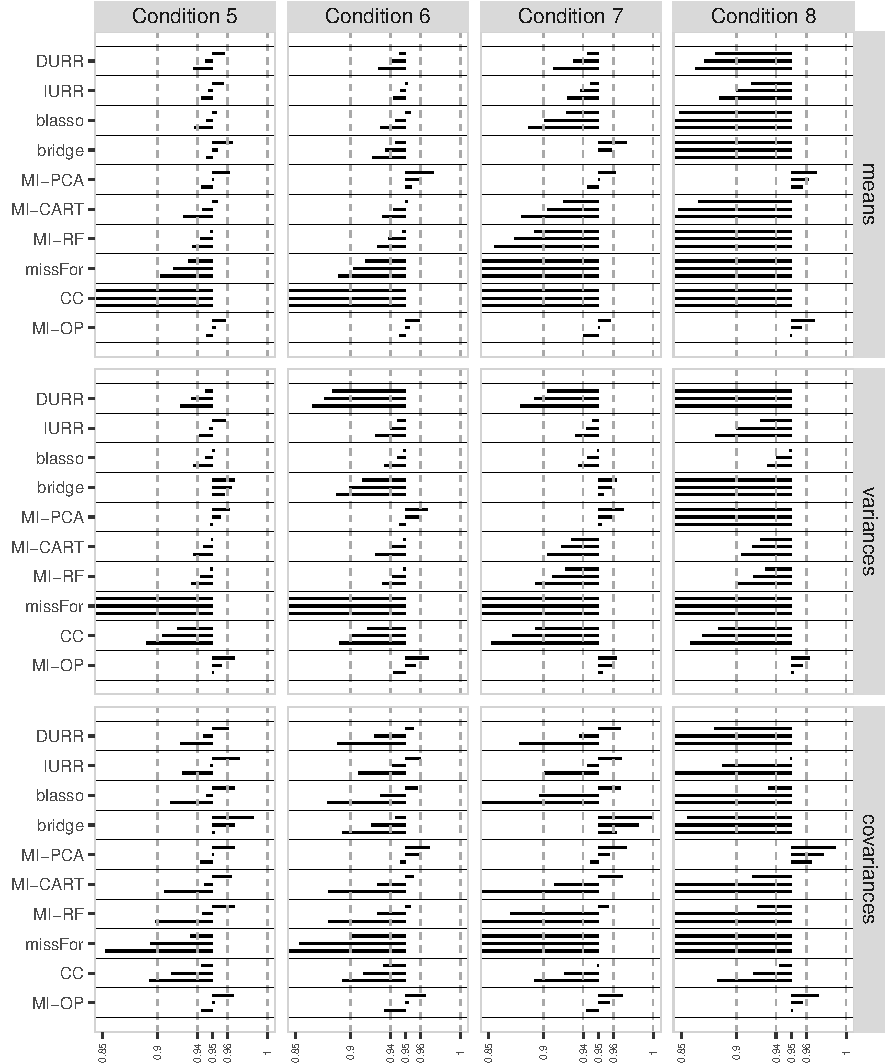
\includegraphics{../../output/graphs/exp2_semR_ci_58_summy.pdf}
\caption{CIC for the means, variances, and covariances for condition 1 to 4.
	For every method, single horizontal lines, representing the CIC of a parameter estimate on 
	a single variable (or pair of variables), combine to form larger horizontal bars giving an 
	aggregate account of how each method performed across multiple variables with missing values.
}
\label{fig:exp2cir58}
\end{figure}

\FloatBarrier

	\paragraph{Factor Loadings}
	Figure \ref{fig:exp2fl14} shows the average, minimum, and maximum PRB values for all the factor loadings 
	estimated by the Confirmatory Factor Analysis described above. 
	Most MI-Methods provided acceptably low bias for these estimates in all conditions except the one with 
	both large proportion of missing values and high dimensional input data matrix (condition 4 and 8).
	MI-OP, IURR, and MI-PCA outperformed all other methods and produced virtually unbiased estimates
	of the factor loadings in all conditions.
	In particular, MI-PCA outperformed IURR when factor loadings were low (panel b), 
	maintaining inconsequential biases even when data were high-dimensional and the proportion of missing 
	values was high.

\begin{figure}
	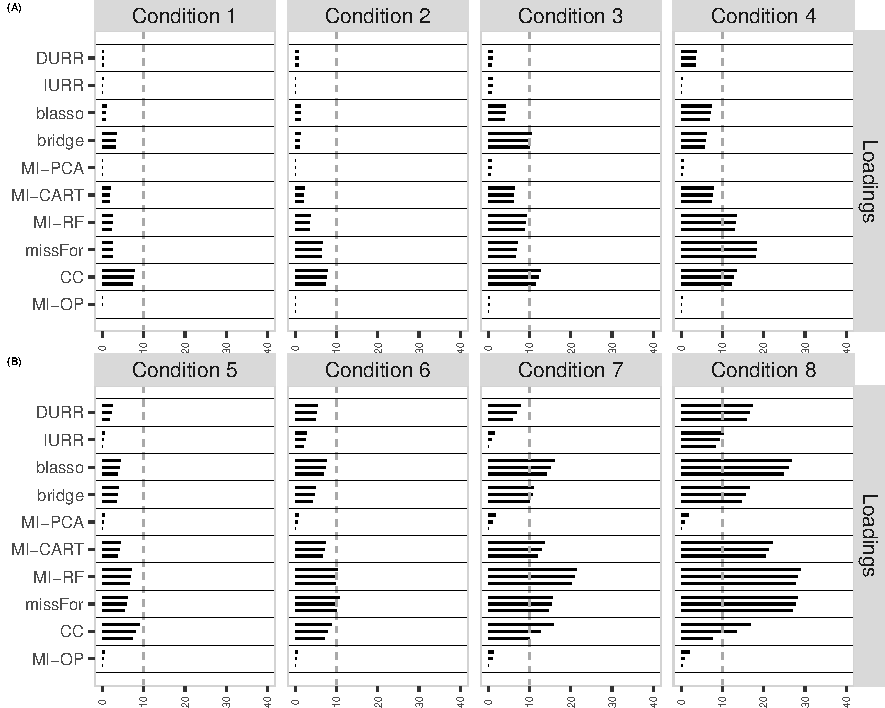
\includegraphics{../../output/graphs/exp2_CFA_lambda_BPR_summy.pdf}
	\caption{
		Percent Relative Bias (PRB) for the factor loadings in conditions 1 to 4 (panel A) 
		and conditions 5 to 8 (panel B).
		Within each panel, for every method, single horizontal lines report the PRB of the 
		factor loading estimation for each item with missing values.
		}
\label{fig:exp2fl14}
\end{figure}

\FloatBarrier % stops fig:exp2fl to leave its section

